% arara: pdflatex: { interaction : nonstopmode }
% arara: biber: { options: ['--isbn-normalise'] }
\documentclass[t, aspectratio=169, english, table]{_style/tudelft-beamer}
% \includeonlyframes{current}% beamer documentation \S 4.3.3

\title[Git Tutorial]{How to use Git for the LELEC210X project}
\subtitle{About how Git can be your best friend}
\author[Assistants Team\inst{1}]{The LELEC210X Assistants\inst{1}.}
\date{29-01-2024}
% define a graphic to be shown next to the title
\titlegraphic{
\includegraphics[width=0.35\paperwidth]{figures/git.pdf}}

% optional:
% \setlength{\titlesplitpos}{-0.5\paperwidth}
% mind that in this case, the white pane is the background, and the blue one on top.

\institute[Universities of Somewhere and Elsewhere]{
  \strut\llap{\inst{1}\,}UCLouvain}
\date[LELEC210X]{Project in Electrical Engineering, LELEC210X}

\newcommand{\absimage}[4][0.5,0.5]{%
	\begin{textblock}{#3}%width
		[#1]% alignment anchor within image (centered by default)
		(#2)% position on the page (origin is top left)
		\includegraphics[width=#3\paperwidth]{#4}%
\end{textblock}}


\begin{document}


\titleframe


\begin{frame}
  \frametitle{What is Git?}
  \framesubtitle{Git is a versioning tool}
  
  \begin{figure}
    \centering
    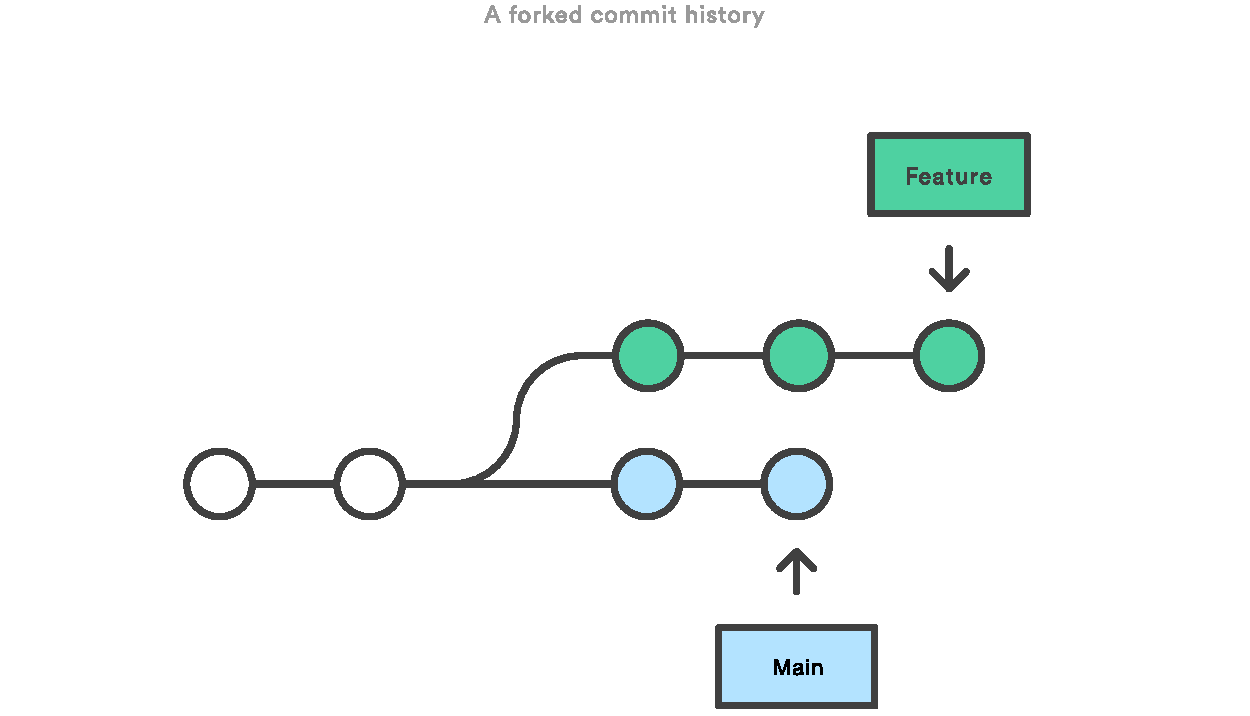
\includegraphics[height=.7\paperheight]{figures/01_git_tree.pdf}
  \end{figure}
  
\end{frame}

\begin{frame}
  \frametitle{What is Git?}
  \framesubtitle{Git can compare files between versions}
  
  \begin{figure}
    \centering
    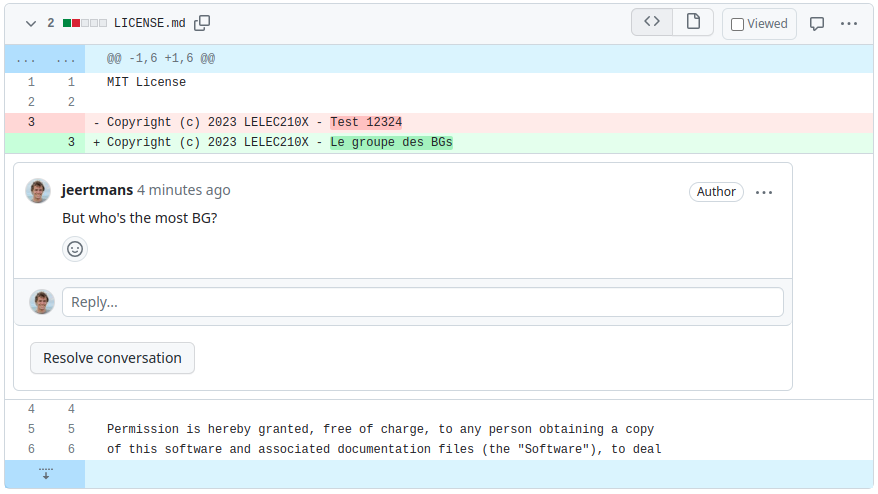
\includegraphics[height=.6\paperheight]{figures/git-diff-comment.png}
  \end{figure}
  
\end{frame}

\begin{frame}
  \frametitle{What is Git?}
  \framesubtitle{Git uses its own language}

  Get to know Git and the following concepts:

  \begin{itemize}
      \item Staging and committing files;
      \item Pulling and pushing changes;
      \item Git branches;
      \item Clone and Fork;
      \item Remotes;
      \item Merge and rebase.
  \end{itemize}

  Checkout this project's \href{https://github.com/LELEC210X/LELEC210X}{\color{tud primary}README} for useful links.
  
\end{frame}

\begin{frame}
  \frametitle{Credits}
  
  Git tree images were taken from Atlassian's guide: \url{https://www.atlassian.com/git/tutorials/merging-vs-rebasing}.
\end{frame}

\begin{frame}
  \frametitle{Git Tools}
  \framesubtitle{We recommend using GitKraken}
  
  \begin{figure}
    \centering
    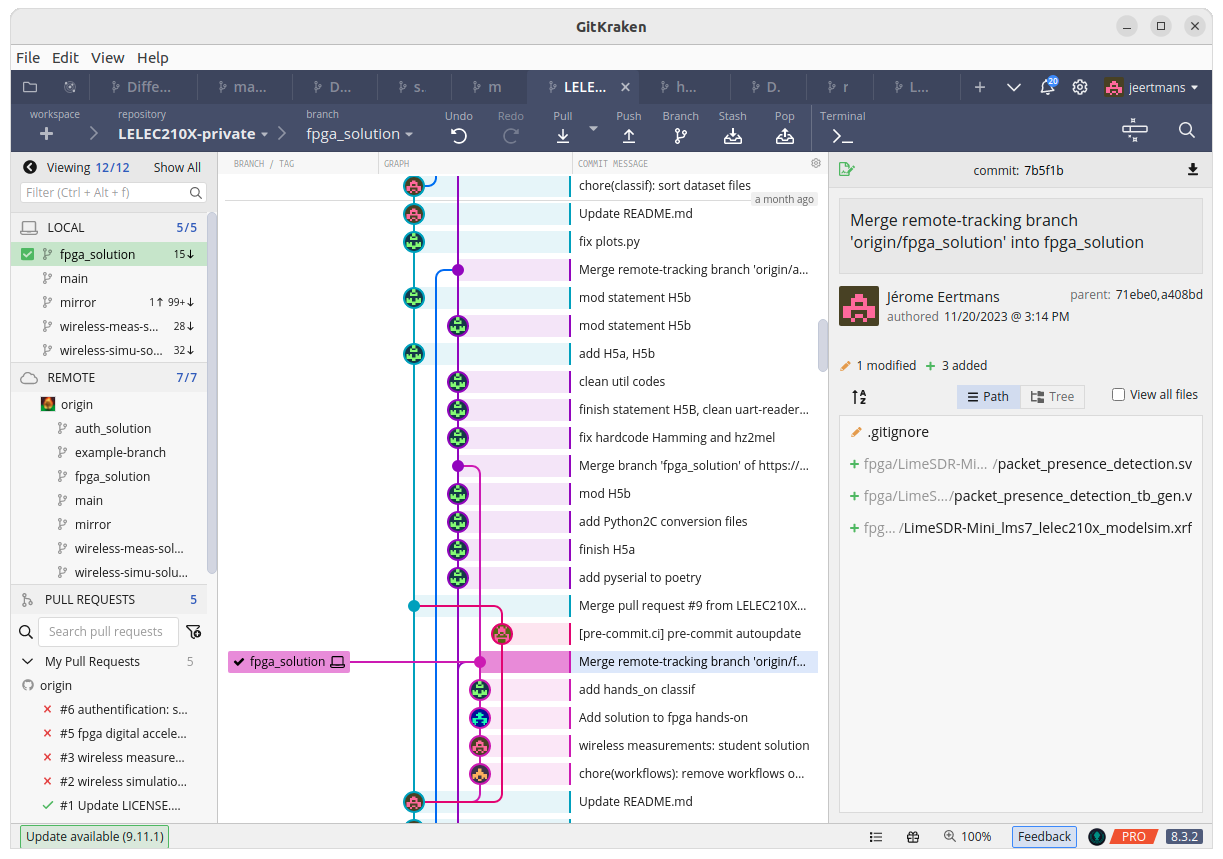
\includegraphics[height=.6\paperheight]{figures/gitkraken.png}
  \end{figure}
  
\end{frame}

\begin{frame}
  \frametitle{How to sync your work}
  \framesubtitle{The basic structure}
  
  \begin{figure}
    \centering
    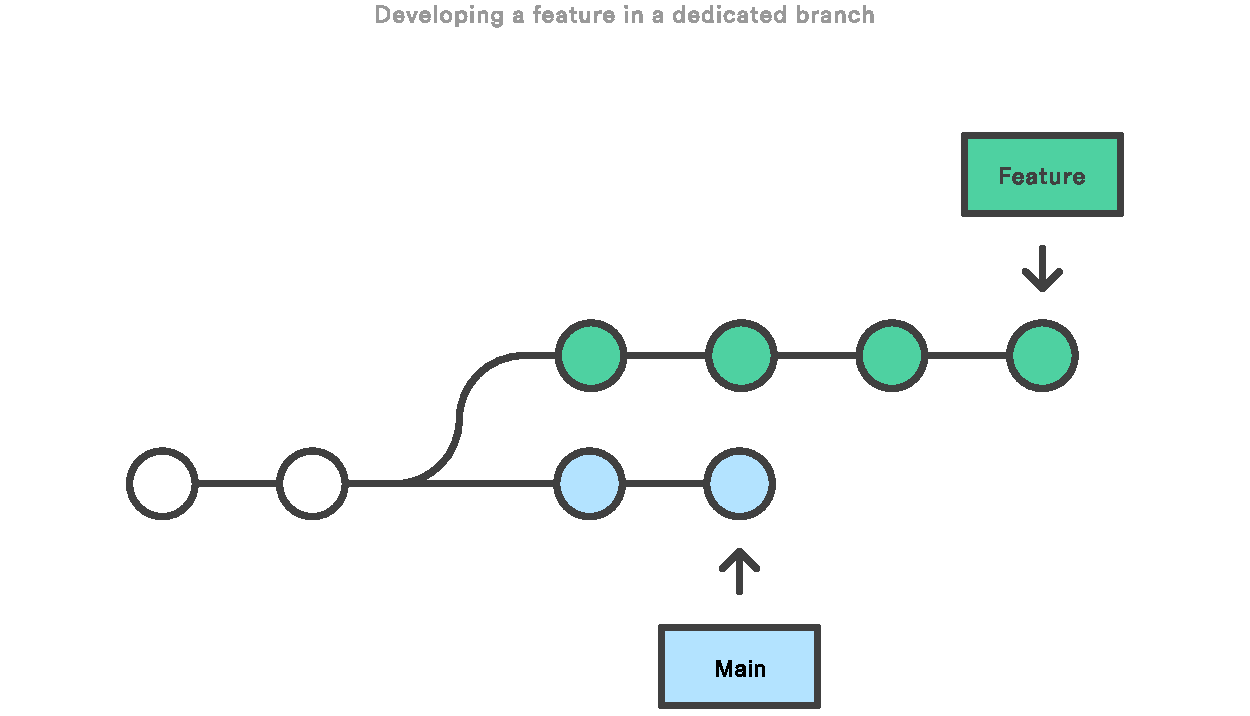
\includegraphics[height=.6\paperheight]{figures/01_basic_git_tree.pdf}
  \end{figure}
  
\end{frame}

\begin{frame}
  \frametitle{How to sync your work}
  \framesubtitle{Merging new changes}
  
  \begin{figure}
    \centering
    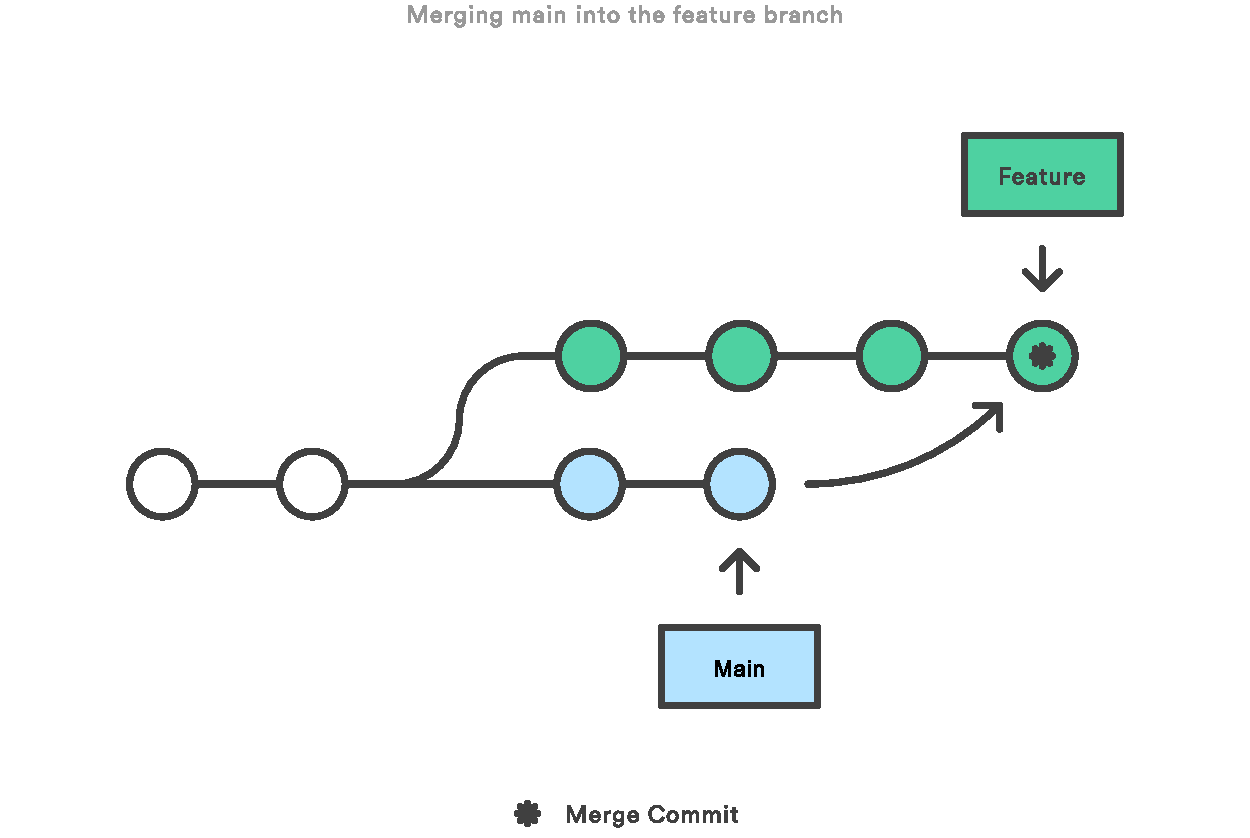
\includegraphics[height=.6\paperheight]{figures/02_merging.pdf}
  \end{figure}
  
\end{frame}

\begin{frame}
  \frametitle{How to sync your work}
  \framesubtitle{Rebasing history}
  
  \begin{figure}
    \centering
    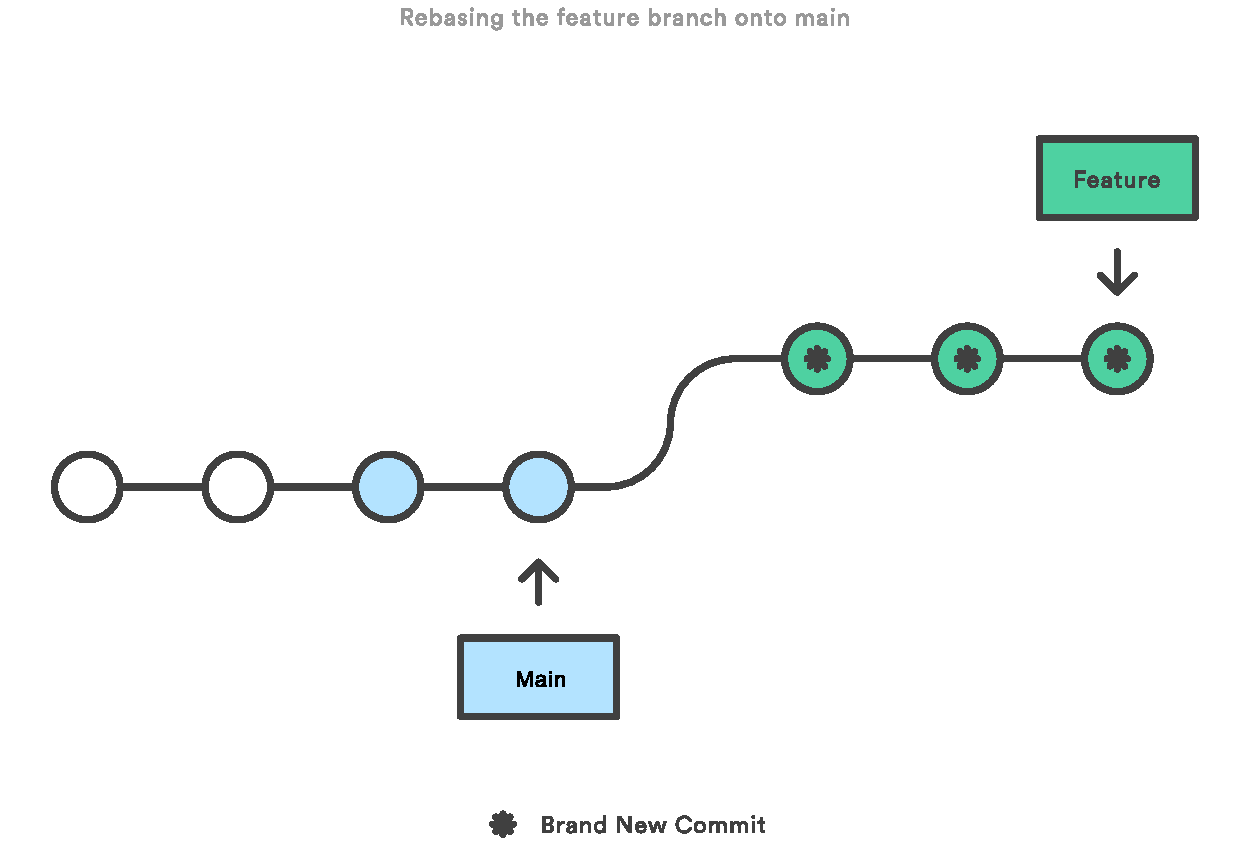
\includegraphics[height=.6\paperheight]{figures/03_rebasing.pdf}
  \end{figure}
  
\end{frame}

\begin{frame}
  \frametitle{How to sync your work}
  \framesubtitle{Synchronizing your work with our repository}
  
  \begin{figure}
    \centering
    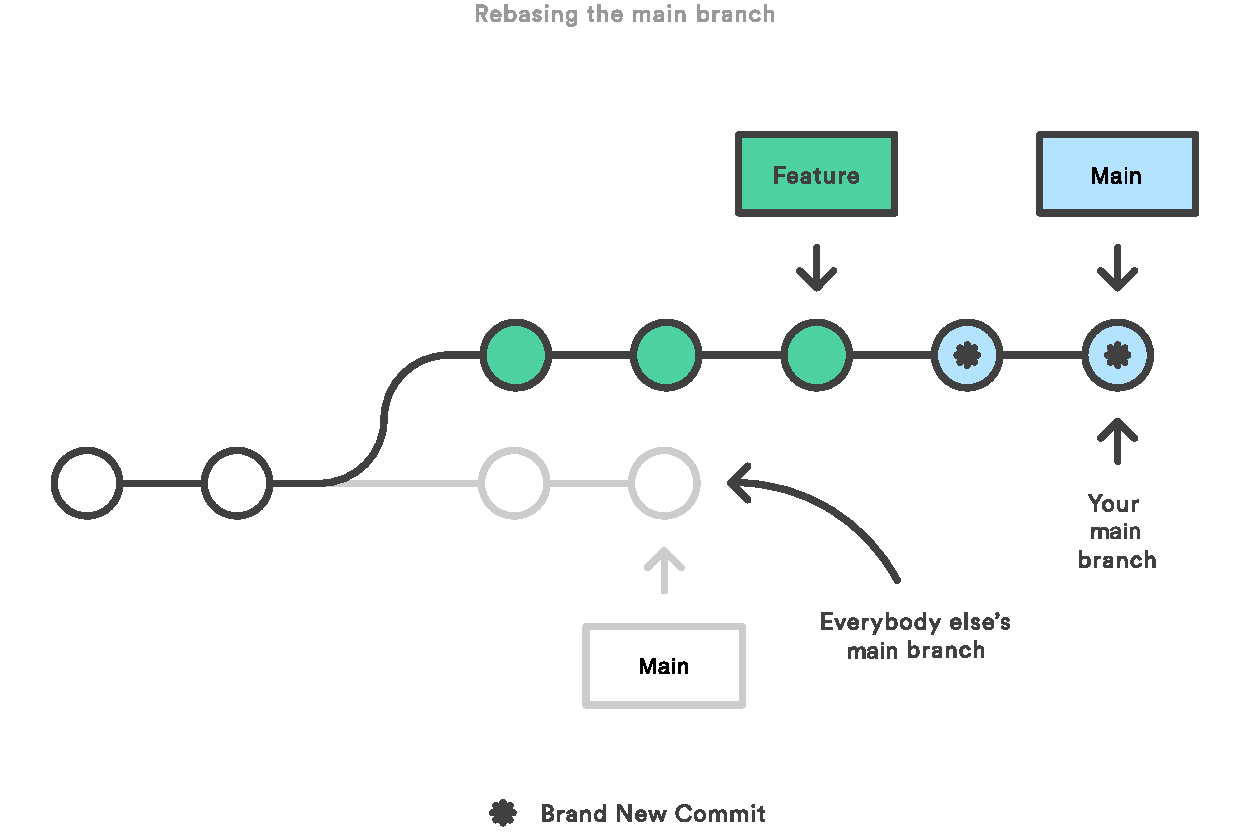
\includegraphics[height=.6\paperheight]{figures/04_rebasing_main.pdf}
  \end{figure}
  
\end{frame}

\begin{frame}
  \frametitle{Live demo}
  \framesubtitle{Working with your own private fork}

  \begin{enumerate}
    \item Clone \href{https://github.com/LELEC210X/LELEC210X}{\color{tud primary}LELEC210X/LELEC210X};
    \item Delete origin remote and create a new (private) one:  \href{https://github.com/jeertmans/LELEC210X}{\color{tud primary}jeertmans/LELEC210X};
    \item Hard reset \texttt{main} branch and force push;
    \item Add a new remote (e.g., \texttt{assistants}) for \href{https://github.com/LELEC210X/LELEC210X}{\color{tud primary}LELEC210X/LELEC210X};
    \item Create branch \texttt{feature}, add new dummy file, commit, push and create pull request (PR);
    \item Review PR, accept, and merge \texttt{feature} into \texttt{main}.
    \item Create and push 5 commits to \texttt{origin/main} changes conflicting with \texttt{assistants/main};
    \item Rebase \texttt{origin/main} onto \texttt{assistants/main} and push changes;
    \item Redo previous step, but merge instead to see the differences.
  \end{enumerate}
\end{frame}


\end{document}
